% ---------------------------------------------------------------------------- %
\chapter{Speech}
\label{ch:speech}
% ---------------------------------------------------------------------------- %
Language is a system that allows humans to communicate an unlimited combination
of ideas using an highly structured stream of sounds or manual and facial
gestures~\citep{kandel.schwartz.jessel:2000}.
At the end of the Ninetieth century, Paul Broca investigated the anatomical
lesions in the left hemisphere that, according to Marc Dax, led to aphasias.
According to Broca, the language impairment that appeared in aphasic patients
was justified by the loss of the faculty of coordinating meaningless
articulatory gestures during vocalization.
In other words, the higher-level faculty of language relies on speech, that is,
the act of producing voice trough the use of the vocal apparatus.

As explained in the previous Chapter, the role of the Broca's area is not
limited to speech, but also to gesture recognition
(Section~\ref{sec:actions:human}).
For example, Broca's area becomes active during the observation of hand shadows 
mimicking animals opening their mouths, and for this reason it might function as
a ``motor assembly system, which links and interprets motor sequences for
both speech and hand gestures''~\citep{fadiga.etal:2006}.

The ``Motor Theory of Speech Perception'' claims that the real objects of speech
are the phonetic gestures of the speaker.
Those gestures are represented in the brain as invariant motor commands and,
during vocalization, are translated in significant configurations of the
articulators~\citep{liberman.mattingly:1985}.
Keeping in mind the theoretical framework proposed by Liberman and Mattingly, 
\citet{rizzolatti.arbib:1998} hypothesized that the mirror neurons on monkey's
F5\comment{that links the observer and the actor,} could be evolved in a
modern system devolved to communication that links the sender and the receiver
of a certain message.

This Chapter aims to briefly describe what language is by presenting the
classical Wernicke-Geschwind model 
(Section~\ref{sec:speech:language}) and to show how the
different articulators are involved in speech production by describing their 
anatomical properties (Section~\ref{sec:speech:language:mechanism}).
The overview of the articulatory mechanism is not omni-comprehensive. In fact,
the author highlights only the aspects that play a crucial role in the task of
acquiring phono-articulatory features for the CONTACT Project
(Chapter~\ref{ch:linguometer}).
Finally, at the end of this Chapter the author presents an overview of the 
recent works that hypothesize that speech and manipulation abilities
are tightly coupled from both a neurophysiological and an evolutionary
perspective (Section~\ref{sec:speech:mirror}).
% ---------------------------------------------------------------------------- %
\section{Language}
\label{sec:speech:language}
% ---------------------------------------------------------------------------- %
Language is relies on two main components: \emph{words} and \emph{grammar}. 
A word is an arbitrary association between a sound and a meaning, while grammar
consists in a set of rules that describe how words can be combined in phrases
and sentences.
%Words are commonly used to describe a vast set of concepts, such as objects,
%states, events and places.
The entire set of words known by an individual is known as \emph{vocabulary}. 
On the other hand, grammar is fundamental arrange words in a particular
combination that is necessary to understand the meaning of a message.
The main components of grammar are \emph{morphology}, \emph{syntax} and
\emph{phonology}. The rules of morphology describe how words and affixes could
be combined to form larger word. Syntax describe how to combine words into
phrases and phrases into sentences. Finally, phonology consists in rules that
describe how sounds can be combined together for generating vocalizations
consistent with the spoken language~\citep{kandel.schwartz.jessel:2000}.

Language is the preferred tool for communication in normal humans and its
development requires social interaction~\citep{moskovitz:1978}.
Children spontaneously develop language abilities, producing language-like
sounds between five and seven months of age.
At the age of three, kids use grammatical words correctly most of the time and 
their production performances are comparable with the adults'.
Language and motor abilities develop in parallel, passing trough a series of 
well determined stages~\citep{lennenberg:1967}.
The debate about language development is still open and many different
approaches to the problem have been proposed.
The behaviorist hypothesis suggests that leaning language consists in learning a
vast set of associations~\citep{skinner:1957}.
Since language appears to have a ``universal design'', nativist theories
claim for an innate knowledge of the rules of grammar (the ``universal 
grammar'') that are common to all human languages~\citep{chomsky:1968}.
However, language abilities are not completely innate nor they entirely rely
on learning. 
Surely the ability to acquire language is innate and probably it comes from
``adaptations of the human brain that arose in the course of human
evolution''~\citep{kandel.schwartz.jessel:2000}. 

Humans are the only primates that use such a complex system for social
communication. 
In fact, humans combine a finite set of meaningful elements in oder to generate
an almost infinite set of meanings suitable for describing the physical reality
or even abstract ideas.
On the other hand, non-human communication is based on three designs such as 
a finite repertoire of calls, the modulation of a continuous analog signal and 
a sequence of randomly ordered calls that serve as a variation over a
theme~\citep{kandel.schwartz.jessel:2000}.

During the latest century, lots of efforts have been spent, unsuccessfully, 
teaching human verbal and sign language to primates, mainly 
chimpanzees\footnote{
\citet{marcus:2004} provides a comprehensive review of the many experiments 
conducted from the real beginning of the Twentieth century.}.
Recently, \citet{savage-rumbaugh.etal:1993} focused on perception aspects 
instead of the production ones, discovering that Kanzi, an eight year old
bonobo, was able to decode recursive sentences with higher accuracy than a
two years old child. 
In contrast, the child demonstrated to perform better than Kanzi in decoding
sentences connected by conjunctives (e.g.: and, since, therefore).
At the end of this Chapter, the topic of language evolution is covered,
although the dissertation mainly focuses onto the idea that language evolved
from manipulatory abilities, as proposed
by~\citet{rizzolatti.arbib:1998}.
% ---------------------------------------------------------------------------- %
\subsection{The Wernicke-Geschwind model}
\label{sec:speech:language:wg}
% ---------------------------------------------------------------------------- %
The faculty of language in humans lack of homologue in animals.
For this reason, the study of language was mainly conducted on patients affected
by language disorders, such as \emph{aphasia} (loss of the ability to produce 
and/or comprehend language, due to brain injury).

% ---------------------------------------------------------------------------- %
\begin{figure}[htbp]
	\centering
	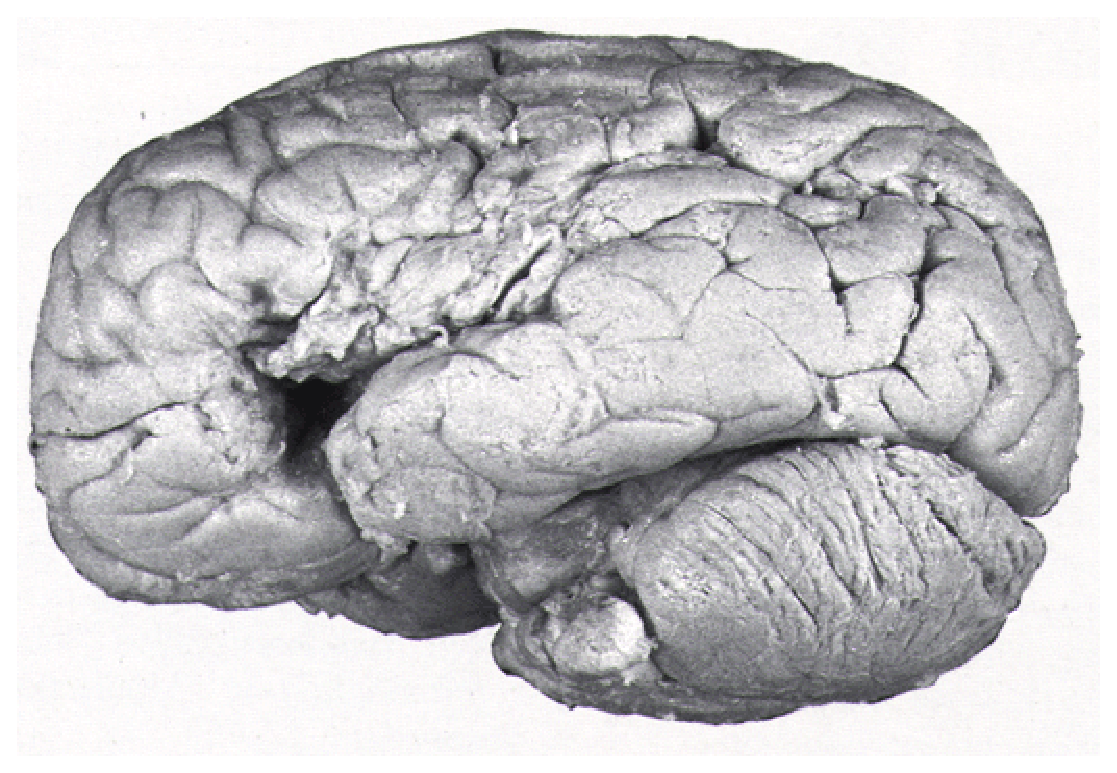
\epsfig{file=include/speech/images/tan.eps, width=0.50\textwidth}

	\caption[Tan's brain]{\textbf{Tan's brain}:
	in 1861 Broca dissected the brain of his patient Leborgned, nicknamed ``Tan''
	due the inability to produce any words other than ``tan''.
	The lesion caused by syphilis in the left cerebral
	hemisphere at the level of Broca's area is clearly visible in the picture.}
	\label{fig:speech:tan}
\end{figure}
% ---------------------------------------------------------------------------- %

At the end of the Ninetieth century, Paul Broca investigated the anatomical
lesions in the left hemisphere that, according to Marc Dax, led to aphasias.
In 1861 Broca dissected the brain of his patient Leborgned, nicknamed ``Tan''
due to the inability to produce any words other than ``tan''.
Broca determined that Tan had a lesion caused by syphilis in the left cerebral
hemisphere, specifically in the ventroposterior region of the frontal lobes
(Broca's area). Figure~\ref{fig:speech:tan} shows a picture of Leborgned's brain
and the lesion at the level of Broca's area.

The early studies on aphasics suggested that in a majority of right and left
handed individuals language processing related to grammar, lexicon, phonemic
assembly and phonetic production depends principally on the left
hemisphere structures.
Also the American Sign Language depends mainly on the left hemisphere, trough it
relies on visuomotor signs rather than auditory speech
signs~\citep{kandel.schwartz.jessel:2000}.

% ---------------------------------------------------------------------------- %
\begin{figure}[htbp]
	\centering
		\epsfig{file=include/speech/images/model.tps, width=0.65\textwidth}

	\caption[Broca's and Wernicke's areas]{\textbf{Broca's and Wernicke's areas.}
	Representation of the simplified Wernicke-Geschwind language processing
	model.
	Broca's area (\textbf{B}) is joined to Wernicke's area by the arcuate
	fasciculus (brown arrow).
	Reproduced from~\citet{kandel.schwartz.jessel:2000}.}
	\label{fig:speech:wg}
\end{figure}
% ---------------------------------------------------------------------------- %

The study of the brain lesions leading to speech disabilities identified two
main cortical areas implied in the processes of speech production and
perception.
The first one, Broca's area, is located on the frontal lateral region, and it
is devolved to the articulation of speech.
The latter one, Wernicke's area, is located in the posterior superior temporal
lobe and is involved in the processing of the acoustic images of speech.
Broca's Area is connected to Wernicke's area by a neural pathway called the 
arcuate fasciculus (Figure~\ref{fig:speech:wg}).
Broca's area comprises BA44 and BA45 and it is subdivided in two main portions:
the anterior \emph{pars triangularis} and the
posterior \emph{pars opercularis}~\citep{kandel.schwartz.jessel:2000}.
Functional evidence suggest that human BA44 contains both speech representation
and motor representation of hand movements, as does area F5 in the macaque 
monkey. 
Those results strongly suggest that human Broca's area is the homologue of
monkey's area F5~\citep{rizzolatti.craighero:2004}.
Neurophysiological investigations reveal that area F5 is agranular while Broca's
area is dysgranular, 
thus suggesting that that a cortical area comparable
in architecture to human area 44 exists in the macaque monkey immediately in 
front of premotor cortical area 6V (inside the inferior arcuate sulcus) and
that it is involved with the orofacial musculature~\citep{petrides.etal:2005}:
\begin{quote}
We suggest that area 44 might have evolved originally as an area exercising 
high-level control over orofacial actions, including those related to 
communicative acts, and that, in the human brain, area 44 eventually also came 
to control certain aspects of the speech act.
\end{quote}
The findings about Broca's and Wernicke's area brought to the development of the
classical Wernicke-Geschwind model of language processing, which is founded on 
three assumptions. 
Firstly, processing is handled by Broca's and Wernicke's areas. 
Secondly, the arcuate fasciculus was thought to be an unidirectional pathway
connecting Wernicke's to Broca's area. 
Lastly, both areas were thought to interact with the polymodal association
cortices \footnote{The association cortices include most of the cerebral
surface of the 
human brain and are largely responsible for the complex processing that goes 
on between the arrival of input in the primary sensory cortices and the 
generation of behavior. 
Inputs to the association cortices include projections from the primary and
secondary sensory and motor cortices, the thalamus, and the brainstem. 
Outputs from the association cortices reach the hippocampus, the basal ganglia
and cerebellum, the thalamus, and other association cortices
\citep{purves.etal:2001}.}.
The Wernicke-Geschwind model provide a useful framework for the classification
of aphasias, although modern studies outstand it in terms of 
complexity\footnote{Recent findings reveal that the role of Broca's and 
Wernicke's areas is not clear as it appears in the Wernicke-Geschwind model.
Moreover, the arcuate  fasciculus is characterized by bidirectional properties
and joins a large set of sensory cortices with prefrontal and premotor cortices.
Lastly, language processing involve higher-order association cortices in the 
left frontal, temporal and parietal 
regions~\citep{kandel.schwartz.jessel:2000}.}.
% ---------------------------------------------------------------------------- %
\subsection{Aphasias}
\label{sec:speech:language:aphasias}
% ---------------------------------------------------------------------------- %
Aphasia is the loss of the ability to produce and/or perceive language correctly
due injuries to specific brain areas. Aphasic patients are normally intelligent
and do not suffer of muscle paralysis.

Broca's aphasia is caused by damage to the frontal lobe of the left hemisphere
of the brain. Subjects with Broca aphasia speak short phrases that require great
effort. 
Subjects with Broca aphasia often have right side paralysis since the injury 
could affect the motor cortex, that is located near by Broca's area.
Subject with Wernicke aphasia do not suffer of paralysis or weakness since the
Wernicke's area is located in the temporal lobe.

Many other types of aphasias have been reported and the classification appears
to be more complex and fine-grained with respect to what is presented in this
Section.
This Section aims to cover the principles of language processing in humans and,
for this reason, just three types of aphasias are discussed.
% ---------------------------------------------------------------------------- %
\subsubsection{Broca aphasia}
\label{sec:speech:language:aphasias:broca}
% ---------------------------------------------------------------------------- %
Broca aphasia is due large frontal lobe lesions involving Broca's area, the
surrounding frontal fields\footnote{BA6, BA8, BA9, BA10 and BA46}, the
underlying white matter, insula, basal ganglia and a small portion of the
anterior superior temporal gyrus. The patient speech is slow and articulation is
impaired. Furthermore, the melodic intonation of speech is
lacking~\citep{kandel.schwartz.jessel:2000}.
If the damage occurred just at the level of BA44 and BA45, the patient develops
a milder aphasia (Broca area aphasia) rather than a true Broca aphasia.
The production of speech is definitely impaired, but aphasics can still
communicate successfully since the selection of words is often correct.
Comprehension is only partial and aphasics loose the ability to repeat complex
sentences spoken by the examiner.
Broca's aphasia is not a production-only deficit. In fact, aphasics cannot
understand complex sentences that rely on complex grammatic structures
(e.g.: recursive sentences). On the other hand, aphasics can infer the meaning 
of simple sentences starting from the meaning of each word.
% ---------------------------------------------------------------------------- %
\subsubsection{Wernicke aphasia}
\label{sec:speech:language:aphasias:wernicke}
% ---------------------------------------------------------------------------- %
Wernicke aphasia is caused by damage to the posterior sector of the left
auditory association cortex (BA22).
In severe cases, lesions extend to the middle temporal gyrus and deep white
matter.
Subjects that suffer of this form of aphasia speak effortless at normal rate 
and the production appears melodic, although they make frequent errors in the 
choice of words and phonemes, leading to unintelligible
words~\citep{kandel.schwartz.jessel:2000}.

Wernicke's area is no longer considered involved in auditory comprehension.
Indeed, the modern view suggest that Wernicke's area constitute the center for 
speech sound processing. 
% ---------------------------------------------------------------------------- %
\subsubsection{Conduction aphasia}
\label{sec:speech:language:aphasias:conduction}
% ---------------------------------------------------------------------------- %
Conduction aphasia results from damage to the left superior temporal gyrus and
the inferior parietal lobe (BA39 and BA40) but the damage may extend to the
primary auditory cortex (BA41 and BA42), the insula and the underlying white
matter. There is no evidence that conduction aphasia is due the damage of the
arcuate fasciculus, although the damage interrupts its projections that connect temporal, parietal, insular and frontal 
cortices~\citep{kandel.schwartz.jessel:2000}.
% ---------------------------------------------------------------------------- %
\section{The articulatory mechanism}
\label{sec:speech:language:mechanism}
The purpose of this Section is to briefly describe the anatomical structures
involved in human speech production (lungs, jaw, lips, hard and soft palate, 
larynx and pharynx, where the vocal folds are located) not paying much
attention to the  phonological aspects of articulation.
The air in the lungs pass trough the pharynx then out trough the oral and the
nasal cavity.
During voiced sounds (vowels) the vocal folds oscillate generating a
quasi-periodic pressure wave. 
In contrast, during the production of unvoiced sounds, the air flow trough the
vocal folds is unobstructed.
The air flow trough the oral cavity is modulated by the position of the lips,
the tongue and the jaw that modulate the deformation of the vocal cavity
resulting in an amplification of attenuation of the different harmonics of the
excitation signal. 
For example, a small constriction of the vocal tract between the tongue and 
the hard palate leads to the production of 
\emph{fricative}\footnote{Fricatives (or spirants):
consonants produced by forcing air trough a narrow channel.} sounds like
\textbf{/s/}.
The rapid release of the air pressure built behind a closure in the oral cavity
leads to high-frequency burst sounds. 
For example, the fast release of the lips cause the emission of the
sound \textbf{/p/}~\citep{blackburn:1996,epstein.etal:2002}.
% ---------------------------------------------------------------------------- %
\subsubsection{The lungs}
Air is pushed in the lungs by the action of different muscles: the
\emph{internal} and the \emph{external intercostals}, the \emph{rectus 
abdominis}, the \emph{external obliques} and the \emph{diaphragm}.
The thoracic cavity can be enlarged by raising the rib cage with the 
external intercostals muscles or by lowering (by contraction) the diaphragm. 
Expiration is a passive process but, during speech, can be modulated by the
expiratory action of the internal intercostal muscles.
If, at the end of an utterance, the intercostals alone cannot produce the
required pressure inside the thoracic cavity, the rectus abdominis and the 
external obliques can push the diaphragm upward 
(Figure~\ref{fig:speech:articulators:lungs}).
% ---------------------------------------------------------------------------- %
\begin{figure}[htbp]
	\centering
		\epsfig{file=include/speech/images/lungs.tps, width=0.30\textwidth}

	\caption[Posterior surface of sternum]{\textbf{Posterior surface of sternum.}
	Reproduced from~\citet{gray:1918}.}	
	\label{fig:speech:articulators:lungs}
\end{figure}
% ---------------------------------------------------------------------------- %

% ---------------------------------------------------------------------------- %
\subsubsection{The jaw}
During speech, the position of the jaw affects the position of the tongue thus
modulating the distance between the tongue and the hard palate.
This distance is involved in the production of
\emph{sibilant}\footnote{Sibilants (or stridents): a subset of fricative
consonants. In addition the tongue is curled lengthwise to direct the air over 
the edge of the teeth.}
consonants such as \textbf{/s/} and \textbf{/z/}.
Furthermore, proper positioning of the jaw plays a fundamental role
in the production of labial consonants.
\comment{(e.g.: \textbf{/p/},
\textbf{/b/}, \textbf{/m/}, \textbf{/f/} and \textbf{/v/})}
Three muscles contribute to jaw closing: the \emph{masseter} elevates and draws
forward the angle of the mandible, the anterior two thirds of
the \emph{temporalis} muscle help the elevation movement and the
\emph{buccinator} pulls back the angle of the mouth and flattens the cheek area
(Figure~\ref{fig:speech:articulators:jaw}).
% ---------------------------------------------------------------------------- %
\begin{figure}
	\centering
	  \subfigure[\label{fig:speech:articulators:jaw:1}]
		{\includegraphics[width=0.35\textwidth]{include/speech/images/jaw_buccinator.tps}}
	  \hspace{0.05\textwidth}
	  \subfigure[\label{fig:speech:articulators:jaw:2}]
		{\includegraphics[width=0.55\textwidth]{include/speech/images/jaw_head.tps}}

	\caption[Muscles of the head, face and neck]{\textbf{Muscles of the head, face and neck.} 
	Reproduced from~\citet{gray:1918}.}	
	\label{fig:speech:articulators:jaw}
\end{figure}
% ---------------------------------------------------------------------------- %

% ---------------------------------------------------------------------------- %
\subsubsection{The lips}
According to~\citet{epstein.etal:2002}, three are the most important movements
of the lips during speech.
The first one is \emph{rounding-spreading}. Rounding occurs when the lips are
drawn together by the action of the \emph{orbicularis oris muscle}
The opposite movement (spreading) occurs when the lips are pulled apart by the
\emph{zygomaticus muscles} (\emph{major} and \emph{minor}), the buccinator and
the \emph{risorius} muscle.
The second movement is \emph{protrusion} and is made protruding the lips to
obtain a longer vocal tract.
The upper lip is controlled by the \emph{levator labii superioris} and by the
zygomaticus minor. On the other hand, the muscles that play a major role in
controlling the lower lip are the \emph{mentalis} and the \emph{depressor
labii oris} (Figure~\ref{fig:speech:articulators:jaw}).
Lastly, the third movement is \emph{compression}, where the lips come together. 
This effect is due the activation of the inferior part or the orbicularis muscle
and the mentalis muscle but can also be achieved raising the jaw.
% ---------------------------------------------------------------------------- %
\subsubsection{The palate}
The soft and hard palate separate the oral cavity from the nasal cavity.
The soft palate is made up by connective tissue and regulates the opening
between the nasopharynx  and the oropharynx.
Specifically, the \emph{tensor palatini muscle} and the \emph{levator palatini
muscle} control the movement of the soft palate.
The hard palate comprises two thirds of the palate and it is made by bone,
as shown in Figure~\ref{fig:speech:articulators:mouth}.
% ---------------------------------------------------------------------------- %
\begin{figure}
	\centering
	  \subfigure[\label{fig:speech:articulators:mouth:1}]
		{\includegraphics[width=0.45\textwidth]{include/speech/images/palate_hardsoft.tps}}
	  \hspace{0.05\textwidth}
	  \subfigure[\label{fig:speech:articulators:mouth:2}]
		{\includegraphics[width=0.35\textwidth]{include/speech/images/mouth_sagittal.tps}}

	\caption[Sagittal view of mouth and palate]{\textbf{Sagittal view of mouth and palate.} 
	Reproduced from~\citet{gray:1918}.}	
	\label{fig:speech:articulators:mouth}
\end{figure}
% ---------------------------------------------------------------------------- %

% ---------------------------------------------------------------------------- %
\subsubsection{The pharynx, the larynx and the vocal folds}
The pharynx is the part of the throat situated posterior to the mouth and nasal
cavity and superior to the esophagus.
The \emph{nasopharynx} is nasal part of the pharynx and it is located behind 
and above the soft palate.
The \emph{oropharynx} constitutes the oral part of the pharynx. It
reaches from the soft palate to the level of the hyoid bone
(Figure~\ref{fig:speech:articulators:larynx}).

% ---------------------------------------------------------------------------- %
\begin{figure}[htbp]
	\centering
		\epsfig{file=include/speech/images/vocalfolds.tps, width=0.45\textwidth}

	\caption[Vocal folds]{\textbf{Vocal folds.}
	Reproduced from~\citet{gray:1918}.}	
	\label{fig:speech:articulators:vocalfolds}
\end{figure}
% ---------------------------------------------------------------------------- %

The vocal folds are located inside the larynx, which is situated just below
where the pharynx splits into the trachea and the esophagus
(Figure~\ref{fig:speech:articulators:vocalfolds}).
In this context, the major movements for speech production are: abducting or
adducting, lengthening or shortening, tensing or relaxing the vocal folds and 
raising or lowering the larynx~\citep{epstein.etal:2002}.
Vocal folds adduction is necessary for speech, while abduction happens
during breathing. The length of the vocal folds modulates the pitch of voiced
sounds while their tension modulates phonation.
The vocal folds are attached to the thyroid cartilage (at the front) and to the 
arytenoid cartilages (at the rear). When those two cartilages move, the vocal
folds increase or decrease their length, vibrating at higher or lower
frequencies thus varying the pitch of the voice. 
% ---------------------------------------------------------------------------- %
\begin{figure}
	\centering
	  \subfigure[\label{fig:speech:articulators:larynx:1}]
		{\includegraphics[width=0.40\textwidth]{include/speech/images/larynx_frontal.tps}}
	  \hspace{0.05\textwidth}
	  \subfigure[\label{fig:speech:articulators:larynx:2}]
		{\includegraphics[width=0.45\textwidth]{include/speech/images/larynx_behind.tps}}

	\caption[Antero-lateral and posterior view of the larynx]{\textbf{Antero-lateral and posterior view of the larynx} 
	Reproduced from~\citet{gray:1918}.}	
	\label{fig:speech:articulators:larynx}
\end{figure}
% ---------------------------------------------------------------------------- %

% ---------------------------------------------------------------------------- %
\subsubsection{The tongue}
The tongue is made of skeletal muscles and its \emph{dorsum}\footnote{Dorsum:
upper surface} can be divided in two parts.
The first one is the \emph{oral part} and it comprises the first two thirds of
the tongue. The \emph{pharingeal part} faces back to the oropharynx.
Two groups of muscles play a crucial role for tongue movement:
the \emph{extrinsic muscles}, that originate
outside the tongue and connect it with other structures 
and the \emph{intrinsic muscles}, that lie within the tongue.
Those two groups of muscles are described in the next two paragraphs.

The \emph{genioglossus muscle} forms the bulk of the inferior part of the
tongue. It originates from the mandible and its activation pulls the tongue 
forwards.
On the other hand, the \emph{styloglossus muscle} elevates and pulls the tongue
backwards, connecting the tongue with the styloid process.
The \emph{palatoglossus muscle} can assist the action of the styloglossus.
The \emph{hyoglossus muscle} pulls the tongue downwards while the 
\emph{mylohyoid muscle} raises its body.
The mylohyoid muscle forms the floor of the mouth and it is involved in the
elevation of the hyoid bone, and consequently of the larynx.
% ---------------------------------------------------------------------------- %
\begin{figure}
	\centering
	  \subfigure[\label{fig:speech:articulators:tongue:4}]
		{\includegraphics[width=0.30\textwidth]{include/speech/images/tongue_4.tps}}
	  \subfigure[\label{fig:speech:articulators:tongue:3}]
		{\includegraphics[width=0.35\textwidth]{include/speech/images/tongue_3.tps}}

	\caption[Posterior and lateral view of the tongue muscles]{\textbf{Posterior (intrinsic muscles) and lateral view of the tongue (extrinsic muscles).} 
	Reproduced from~\citet{gray:1918}.}	
	\label{fig:speech:articulators:tongue:b}
\end{figure}
% ---------------------------------------------------------------------------- %


Four are the intrinsic muscles that run along the length of the tongue.
The \emph{superior longitudinal muscle} is located under the dorsum of the
tongue and controls the elevation, the deviation and the retraction of the apex.
The \emph{inferior longitudinal muscle} is joined with the styloglossus muscle
and is located on the inferior sides of the tongue.
The \emph{verticalis muscle} and the \emph{transversus muscle} are located in
the body of the tongue. The first one is connected to the superior and the
inferior longitudinal muscles while the latter is attached to the mucous
membrane.
% ---------------------------------------------------------------------------- %
\begin{figure}
	\centering
	  \subfigure[\label{fig:speech:articulators:tongue:1}]
		{\includegraphics[width=0.35\textwidth]{include/speech/images/tongue_1.tps}}
	  \subfigure[\label{fig:speech:articulators:tongue:2}]
		{\includegraphics[width=0.55\textwidth]{include/speech/images/tongue_2.tps}}

	\caption[Oral cavity and coronal section of the tongue]{\textbf{Anterior view of the oral cavity and coronal section of the tongue (intrinsic muscles).} 
	Reproduced from~\citet{gray:1918}.}	
	\label{fig:speech:articulators:tongue:a}
\end{figure}
% ---------------------------------------------------------------------------- %

% ---------------------------------------------------------------------------- %
\section{Motor role of Broca's area in speech}
\label{sec:speech:mirror}
% ---------------------------------------------------------------------------- %
According to the motor theory of speech
perception~\citep{liberman.mattingly:1985}, the objects of speech are the 
phonetic gestures of the speaker (e.g.: tongue backing, lip rounding, jaw
raising).
Those actions of speech are intended as the elementary events of speech
production and perception. 
According to the theoretical framework proposed by Liberman and Mattingly, these
actions are represented in the brain as invariant motor commands 
and, during vocalization, are translated in significant configurations of the
articulators (Section~\ref{sec:speech:language:mechanism}).
Furthermore, if speech perception and speech production share the same set of
invariants, they must be strictly coupled at the brain level.
According to the authors, this link is not built by learning: on the contrary, 
it is innately specified and requires epigenetic development to be achieved.

\citet{fadiga.craighero.etal:2002} found that during speech listening there is
an increase of MEPs recorded from the tongue muscles, demonstrating that
listening activates brain areas involved in motor control.
The experimenters stimulated the left motor representation of the tongue by the
means of TMS while subjects were passively listening to Italian words and
pseudo-words that involve a certain degree of tongue mobilization.
The verbal stimuli used in the experiment could be grouped in two main sets.
The first set groups stimuli characterized by an high degree of tongue
mobilization such as words /birra/, /carro/ and pseudo-words /berro/,
/marro/\footnote{/bi\textbf{rr}a/, /ca\textbf{rr}o/, 
/be\textbf{rr}o/ and /ma\textbf{rr}o/: labiodental fricative
consonant~\textbf{/rr/}.}.
The latter set contained stimuli characterized by a lower degree of tongue
mobilization such as 
words /baffo/, /beffa/ and pseudo-words /ciffo/,
and /ceffa/\footnote{/ba\textbf{ff}o/, /be\textbf{ff}a/, 
/ci\textbf{ff}o/ and /ce\textbf{ff}a/: lingua-palatal fricative
consonant~\textbf{/ff/}.}.
The MEPs evoked by TMS stimulation reached higher amplitudes when the subjects
were listening to /\textbf{rr}/ stimuli. 
Furthermore, words did evoke an higher response than pseudo-words.
The presented results suggest that speech listening
activates precise motor areas with ah high degree of specificity in
discriminating words and non-words sounds.
The work by \citep{fadiga.craighero.etal:2002} does not prove that the
theoretical framework provided by Liberman and Mattingly matches the way the
human brain handles speech perception. On the other hand, the
acoustic/motor resonance resembles the visual/motor resonance typical of the
visuomotor mirror neurons.
According to~\citet{liberman:1993}\footnote{This quotation can be also found at
the real beginning of \citet{rizzolatti.arbib:1998}.}:
\begin{quote}
In all communication, sender and receiver must be bound by a common
understanding about what counts; what counts for the sender must count for the
receiver, else communication does not occur. Moreover the process of production
and perception must somehow be linked; their representation must, at some point,
be the same.
\end{quote}
Two are the main concepts condensed in the quotation. 
Firstly, both the sender and the receiver must share a common repertoire of
speech-oriented motor actions.
The results of the previous experiment show that the motor system resonates
during speech listening the same way it resonates during observation of motor 
actions.
Secondly, speech production and speech perception must be linked abilities. 
The mirror system links action production and action perception at the very low
level of single visuomotor (or audiomotor) neurons.
The presented considerations, as said before, do not prove Liberman's framework,
but reinforce the idea that speech abilities in human may have evolved from
well-founded motor abilities in primates.
\comment{Eventually, Roy etal}

According to~\citet{rizzolatti.arbib:1998}, language evolved from gestural
communication, an ability where the mirror system plays a fundamental role.
In fact, monkey's mirror neurons discharge both during the observation and the
execution of a specific transitive action.
Furthermore, a subset of F5 mirror neurons discharge during the
observation of mouth movements for communication and
eating~\citep{ferrari.etal:2003}. 
Mirror neurons do not embed just visuomotor properties; in fact, audio-motor
mirror neurons discharge both when an action is made by the monkey and when the
monkey ears the action-specific sound~\citep{kohler.etal:2002}.
In a broader perspective the mirror system creates a link between the actor and 
the observer.
%integrating motor proprioception (?information, ma sarebbe una
%ripetizione?) with other kinds of sensory information.
In this context, the mirror system acts as a neural circuit that allows
unconscious processing of the perceived motor actions.

Broca's area is involved in language processing in both the cases of production
and perception~(Section~\ref{sec:speech:language:wg}).
Recent findings demonstrate that Broca's area becomes active
during action observation~(Section~\ref{sec:actions:human}), thus extending its
evolutionary importance.
As said before,~\citet{rizzolatti.arbib:1998} hypothesize that
speech originated from ancient gestural communication abilities by supporting
the idea that primates mainly used oro-facial gestures for one-to-one 
communication. 
In fact, oro-facial expressions combined with brachio-manual gestures
could have enhanced communications since the sender could reinforce its message
providing an higher level of description making transitive and intransitive
gestures.
Furthermore, oro-facial communication in primates does not embed the same
combinational properties that are common to brachio-manual gestures.
According to ~\citet{rizzolatti.arbib:1998}, the primitive use of vocalization
in
primates was to transmit emotionally relevant messages.
%\footnote{This ability is mediated by brain medial 
%areas~\citep{kandel.schwartz.jessel:2000}.}
When a strong link was estabilished between the brachio-manual and the
oro-facial 
communication systems, the control of vocalization gained further importance
since the early utterances did need to be repeatable in order to be imitated.
For this reason, the old control system was inadequate.
A ``Broca's area F5-like precursor'' with mirror properties may have been the
right choice for the control of the novel oro-laryngeal movements.
Manual gestures gradually lost their primitive importance in communication, but 
are still widely used in to enrich the message transmitted by the sender.
A recent study, here presented, investigated the role of Broca's area in both
the fields of speech and motor actions.

In subjects with large lesions involving Broca's area, speech production and
speech perception are impaired, although this is valid just for complex
sentences, since single words perception is not totally
impaired.
In order to verify this claim, 
\citet{fadiga.etal:PRESS} administered single TMS pulses in correspondence of
BA44 while subjects where performing a \emph{phonological 
priming}\footnote{Phonological priming: a target word preceded by a prime that
share with the target the last syllable is recognized faster than the word by 
itself (e.g.: roccia, doccia; palla, stalla). The facilitation in recognition is
referred as \emph{phonological priming effect}.} task. 
Subjects where asked to listen to pairs of stimuli, both words and pseudo-words 
(e.g.: W-W, W-PW, W-PW and PW-PW). 
For certain pairs, the target and the prime did share the last syllable (priming
effect). In some trials, a single TMS pulse was administered between the prime
and the target.
In trials where BA44 functionality was not blocked by TMS pulses, the
experimenters found that the lexical content is crucial for the emergence of the
priming effect\footnote{1. The phonological priming effect appeared 
for stimuli such as W-W, W-PW, PW-W. 
2. Furthermore, no priming effect was present for PW-PW pairs.
3. Lastly, the subject response was faster during W-W and W-PW pairs.} (e.g.:
priming effect for pairs W-W, PW-W and W-PW; no priming effect for PW-PW pairs).
According to the authors, this last result demonstrate that the phonological
priming effect is not a phonological-only effect, since it can not be
observed when the prime-target pair does not contain lexical entries.
During TMS trials, the priming effect was suppressed for the W-PW pairs thus
confirming that Broca's area is not involved in phonological processing of the
stimuli. 
In particular, Broca's area may be involved in supramodal syntactic processing.
%provides access to the lexical content of the
%prime 

In order to verify this very last claim, the authors point out that subjects
suffering of Broca aphasia should also suffer of more broad motor
deficits.
Videos representing biological actions (e.g.: hand grasping a bottle, man
opening a door) and non-biological moving objects (e.g.: a bike falling on the 
ground) have been shown to agrammatic patients impaired by Broca
aphasia and to healthy subjects\footnote{Unpublished results (Fazio et al.) 
described in~\citet{fadiga.etal:PRESS}}.
Later on, the patients were asked to place in the correct temporal order four
frames extracted from the previously observed in the videos (e.g.: man
approaching the door, man moving the hand toward the door handle, man acting
on the handle, man opening the door).
The results demonstrate that aphasics were slower than the
control group. Moreover, aphasics perform better in terms of accuracy on 
non-biological sequences, while the opposite is true for the control group.


